\documentclass[aspectratio=169,11pt,hyperref={colorlinks=true}]{beamer}
% https://github.com/zr-tex8r/BXcjkjatype/blob/master/README-ja.md
\usepackage[whole]{bxcjkjatype}
\usetheme{boxes}
\setbeamertemplate{navigation symbols}{}
\definecolor{suse}{RGB}{2, 211, 95}
\definecolor{susedark}{RGB}{13, 44, 64}
\setbeamercolor{titlelike}{fg=suse}
\setbeamercolor{structure}{fg=suse}
\hypersetup{colorlinks,urlcolor=suse}
\setbeamertemplate{footline}[frame number]
% Inserting graphics
\usepackage{graphicx}
% Side-by-side figures, etc
\usepackage{subfigure}
% Code snippits
\usepackage{listings}
% Color stuff
\usepackage{color}
% underline
\usepackage{soul}

\usepackage{amsmath}
\usepackage{tikz}
\newcommand\RBox[1]{%
  \tikz\node[draw,rounded corners,align=center,] {#1};%
}
\usepackage{hyperref}
%\usecolortheme{buzz}
%\usecolortheme{wolverine}
%\usetheme{Boadilla}
\usepackage[T1]{fontenc}
%\usepackage{fontspec}
%\usepackage[expert, deluxe]{otf}

\definecolor{mygreen}{rgb}{0,0.6,0}
\definecolor{mygray}{rgb}{0.5,0.5,0.5}
\definecolor{mymauve}{rgb}{0.58,0,0.82}


%\usepackage{CJK}
%\pdfmapline{=genshingothic@Unicode@ <genshingothic.ttf}
% bxcjkjatype
%\setgothicfont[<ID>]{<フォントファイル名>}
%\setgothicfont{/Users/foo/Library/Fonts/genshingothic.ttf}
%\setgothicfont{/Users/foo/Library/Fonts/NotoSansCJKjp-Regular.otf}
%\setgothicfont{/Users/foo/Downloads/genshingothic-20150607/GenShinGothic-P-Normal.ttf}
%\setgothicfont{/Users/foo/Downloads/genshingothic-20150607/GenShinGothic-Regular.ttf}
%\setgothicfont{hiragino.ttc}
\setgothicfont{mplus-1p-regular.ttf}
\setCJKfamilydefault{\gtdefault}
%\setCJKfamilydefault{\mcdefault}
%\CJKforce{abcdefghijklmnopqrstuvwxyzABCDEFGHIJKLMNOPQRSTUVWXYZ}


\lstset{%
  backgroundcolor=\color{susedark},   % choose the background color; you must add \usepackage{color} or \usepackage{xcolor}
  breakatwhitespace=false,         % sets if automatic breaks should only happen at whitespace
  breaklines=true,                 % sets automatic line breaking
  captionpos=b,                    % sets the caption-position to bottom
  commentstyle=\color{suse},  % comment style
  extendedchars=true,              % lets you use non-ASCII characters; for 8-bits encodings only, does not work with UTF-8
  keepspaces=true,                 % keeps spaces in text, useful for keeping indentation of code (possibly needs columns=flexible)
  keywordstyle=\color{blue},       % keyword style
%  otherkeywords={*,...},           % if you want to add more keywords to the set
  numbersep=5pt,                   % how far the line-numbers are from the code
  numberstyle=\tiny\color{mygray}, % the style that is used for the line-numbers
  rulecolor=\color{white},         % if not set, the frame-color may be changed on line-breaks within not-black text (e.g. comments (green here))
  showspaces=false,                % show spaces everywhere adding particular underscores; it overrides 'showstringspaces'
  showstringspaces=false,          % underline spaces within strings only
  showtabs=false,                  % show tabs within strings adding particular underscores
  stringstyle=\color{suse},   % string literal style
}

\setbeamerfont{caption}{series=\normalfont,size=\fontsize{6}{8}}
%\setbeamerfont{caption}{series=\normalfont,size=\large}
\setbeamertemplate{caption}{\raggedright\insertcaption\par}

\setlength{\abovecaptionskip}{0pt}
\setlength{\floatsep}{0pt}

\author[Dong Ma, Samuel de Medeiros and Masayuki Igawa]{%
  \texorpdfstring{%
    \centering
    Masayuki Igawa\\
    \href{mailto:masayuki@igawa.io}{masayuki@igawa.io}\\
    \href{https://twitter.com/masayukig}{@masayukig}
  }
  {Dong Ma, Samuel de Medeiros and Masayuki Igawa}
}

\date{19 August, 2017}
\def\place#1{\def\@place{#1}}
\place{\href{https://www.ospn.jp/odc2017/}{@Open Developers Conference 2017 Tokyo}}

\title[Non-Native-English-Speaker
\hspace{2em}\insertframenumber/\inserttotalframenumber]{OpenStackコミュニティにおける\\非英語ネイティブ話者の苦悩と奮闘記}

\setbeamercolor{background canvas}{bg=susedark}
\setbeamercolor{titlelike}{fg=white}
\setbeamercolor{structure}{fg=white}
\setbeamercolor{normal text}{fg=white}
\begin{document}

{%
% \setbeamertemplate{background canvas}{\includegraphics[width=\paperwidth,height=\paperheight]{background_title.png}}
\setbeamertemplate{footline}{}
\setbeamercolor{background canvas}{bg=susedark}
\begin{frame}[noframenumbering]
  \hypersetup{colorlinks,urlcolor=suse}
  \setbeamercolor{author}{fg=white}
  \setbeamercolor{date}{fg=white}
  \setbeamercolor{place}{fg=white}
  \titlepage{}
  \centering
  \@place \par
  \href{https://github.com/masayukig/non-native-english-speaker/tree/odc-2017}{github.com/masayukig/non-native-english-speaker/tree/odc-2017}\\
  \vspace{1em}
  \begin{flushright}
    \tiny\href{https://creativecommons.org/licenses/by/4.0/}{This work
      is licensed under a Creative Commons Attribution 4.0
      International License.}~
\includegraphics[scale=0.3]{cc_by.png}
  \end{flushright}
\end{frame}
}

% \section{Agenda}
% \begin{frame}
%   \frametitle{Agenda}
%   \begin{itemize}
%     \item 自己紹介
%     \item Agenda
%       \item Challenges/Experiences
%       \item Overcoming obstacles
%       \item Onboarding newcomers
%       \item Cultural Challenges
%     \item まとめ
%   \end{itemize}
% \end{frame}

\section{Introduction}
\begin{frame}
  \frametitle{Disclaimer}
  \begin{itemize}
    \item 本資料は、個人の見解です。
    \item 所属する企業・団体を代表する意見ではありません。
  \end{itemize}
\end{frame}

\begin{frame}
  \frametitle{Who am I?}
  \begin{itemize}
    \item Company:SUSE/ノベル株式会社
      \begin{itemize}
        \item QE(Quality Engineering) Team
        \item[] (日本にいるのは私だけ)
        \item \href{https://www.suse.com/newsroom/post/2016/suse-acquires-openstack-iaas-and-cloud-foundry-paas-talent-and-technology-assets-from-hpe-to-accelerate-growth-and-entry-into-new-markets/}{SUSE Acquires OpenStack IaaS and Cloud Foundry PaaS Talent and Technology Assets from HPE to Accelerate Growth and Entry into New Markets}
      \end{itemize}
    \item Job: Senior Software Engineer/Open Source Programmer
      \begin{itemize}
        \item \href{https://www.openstack.org/}{OpenStack}
         \href{https://wiki.openstack.org/wiki/QA}{QA} Upstream development, Core Reviewer
        \item[] (\href{https://docs.openstack.org/developer/tempest/}{Tempest},
         \href{http://status.openstack.org/openstack-health/}{OpenStack-Health},
         \href{https://docs.openstack.org/developer/subunit2sql/}{Subunit2SQL},
         \href{https://docs.openstack.org/developer/stackviz/}{Stackviz})
        \item \href{http://stackalytics.com/?user_id=igawa&release=all&metric=all}{stackalytics.com/?user\_id=igawa}
        \item \href{https://github.com/masayukig}{github.com/masayukig}
      \end{itemize}
  \end{itemize}
\end{frame}

\subsection{Culural Challenges}
\begin{frame}
  \bf\Huge{Culural Challenges}
\end{frame}

\begin{frame}
\frametitle{Japanese}
  \begin{itemize}
    \item 明確に「Yes / No」を言わない
    \item 完璧であろうとする
    \item フラットな話し方
    \item 大きな経済規模→海外に出ていく必要性が薄い
    \item 英語学習は読み書きに重点
    \item 発音・文法が全く異なる
      \begin{itemize}
      \item ``L'' vs ``R'' in words
      \item Subject-Verb-Object (E) vs Subject-Object-Verb (J)
      \end{itemize}
    \item 漢字, ひらがな, カタカナ
      \begin{itemize}
      \item カタカナ: ``ネットワーク'' = ``Network'' (English)
      \item Network(ネットワーク), File(ファイル), Comment(コメント), etc..
      \end{itemize}
    \item 和製英語: Paso-con(パソコン), Air-con(エアコン), Auto-bi(オートバイ)
      \begin{itemize}
        \item \url{https://en.wikipedia.org/wiki/Wasei-eigo}
      \end{itemize}
  \end{itemize}
\end{frame}

\begin{frame}
\frametitle{Chinese - Dong}
  \begin{itemize}
  \item 儒教文化
  \item 可能な限り「Yes」と言う。なるべく「No」は言わない
  \item 「交渉」よりも「聴く」ことを好む
  \item 中国人の発音は、なかなか理解してもらえないことが多い
  \item 文法が異なる
  \item 文章を書く・話すのは、なかなか難しい(文法)
  \end{itemize}
\end{frame}

\begin{frame}
\frametitle{Brazilian - Samuel}
  \begin{itemize}
  \item 英語と近い言語
  \item 短い・直接的な回答はちょっとつまらなく感じる
  \item ``i'' (ポルトガル語) は ``e'' (英語) として発音される
  \item 文法:形容詞が名詞の後ろに来るのが一般的
  \item いくつかの発音は、ポルトガル語に存在しない, e.g ``th'' vs ``f''
  \item 一般的な学校の英語教育レベルは高くない
  \end{itemize}
\end{frame}


\subsection{Language Challenges}
\begin{frame}
  \bf\Huge{Language Challenges}
\end{frame}

\begin{frame}
\frametitle{Reading}
  \begin{itemize}
  \item 最も習得しやすいスキル(一般的には)
  \item 一番重要
  \item IRC(テキストチャット) の会話はあっという間に進む
  \item 長いE-mail, 結論がよくわからない
  \end{itemize}
\end{frame}

\begin{frame}
\frametitle{Writing}
  \begin{itemize}
  \item 文法
  \item 長い、美しい文章を書くのは難しい
  \item シンプルな文章を書くことが広く行われている
  \item IRCなどのチャットのスピード
  \end{itemize}
\end{frame}

\begin{frame}
\frametitle{Listening}
  \begin{itemize}
  \item さまざまなアクセント
  \item スピード
  \item ボキャブラリ
  \item 文法
  \item 様々なノイズのある環境
  \end{itemize}
\end{frame}

\begin{frame}
\frametitle{Speaking}
  \begin{itemize}
  \item ボキャブラリ
  \item 文法
  \item 発音
  \item スピードと流暢さ
  \end{itemize}
\end{frame}

\subsection{Overcoming Obstacles}
\begin{frame}
  \bf\Huge{Overcoming Obstacles}
\end{frame}

\begin{frame}
  \frametitle{Overcoming Obstacles}
  \begin{itemize}
  \item 文化的な課題は、単なる言語の課題よりも克服するのが難しい
  \item 言語に浸る
  \item 限界があるとは思わず、チャレンジ
  \item 可能な限り努力、少しずつ改善されていく
  \item 色々なものを読むことを通じてボキャブラリを増やしていく
  \item 継続・習慣化が大切。毎日少しずつでも効果あり
  \item 便利なツールがたくさん(Google Translate, duolingo, インターネット英会話, etc)
  \item 自分自身、もしくは他の人と練習
  \item まずは、1-to-1の会話から始めるのが無難
  \end{itemize}
\end{frame}

\begin{frame}
\frametitle{Overcoming Obstacles (cont.)}
  \begin{itemize}
  \item[] Reading
    \begin{itemize}
    \item Twitter, Blog, etc. を読む
    \item バイリンガル本を買う (or 同じ本の英語版・日本語版)
    \end{itemize}
  \item[] Writing
    \begin{itemize}
    \item 文通, ブログ, 日記を書く
    \item Twitter
    \item Lang-8 \url{http://lang-8.com/}
    \end{itemize}
  \item[] Listening
    \begin{itemize}
    \item Podcasts
    \item ヒアリングマラソン
    \item TED Talks
    \end{itemize}
  \item[] Speaking
    \begin{itemize}
    \item 友だちを作る
    \item オンライン(Skype等)英会話
    \item Meetup.com \url{https://www.meetup.com/meetup-group-en-jp/}
    \end{itemize}
  \end{itemize}
\end{frame}


\subsection{Onboarding newcomers}
\begin{frame}
  \bf\Huge{Onboarding newcomers}
\end{frame}

\begin{frame}
\frametitle{Newcomers}
  \begin{itemize}
  \item フレンドリー&オープンに
  \item メンターを見つけよう
  \item 意見を共有しよう
  \item 前もって準備しよう
  \item 質問しよう
  \item 英語スキルを常に改善していこう
  \end{itemize}
\end{frame}

\begin{frame}
\frametitle{Native Speakers}
  \begin{itemize}
  \item Be patient(ちょっと我慢して..)
  \item Speak slowly, please(ゆっくり話してください)
  \item Use simple words and sentences(シンプルな言葉・文章を)
  \item Encourage communication(会話を勇気づけて)
  \item Do not make fun(からかわないで)
  \end{itemize}
\end{frame}


\subsection{Questions?}
\begin{frame}
  \frametitle{Questions?}
  \begin{itemize}
  \item[] More Informations
  \item \url{https://opensource.com/article/17/1/non-native-speakers-take-open-source-communities}
  \item \url{https://docs.openstack.org/contributor-guide/non-native-english-speakers.html}
  \end{itemize}
  \begin{center}
    
\includegraphics[width=0.492\textwidth]{world_hands_diversity.png}~
    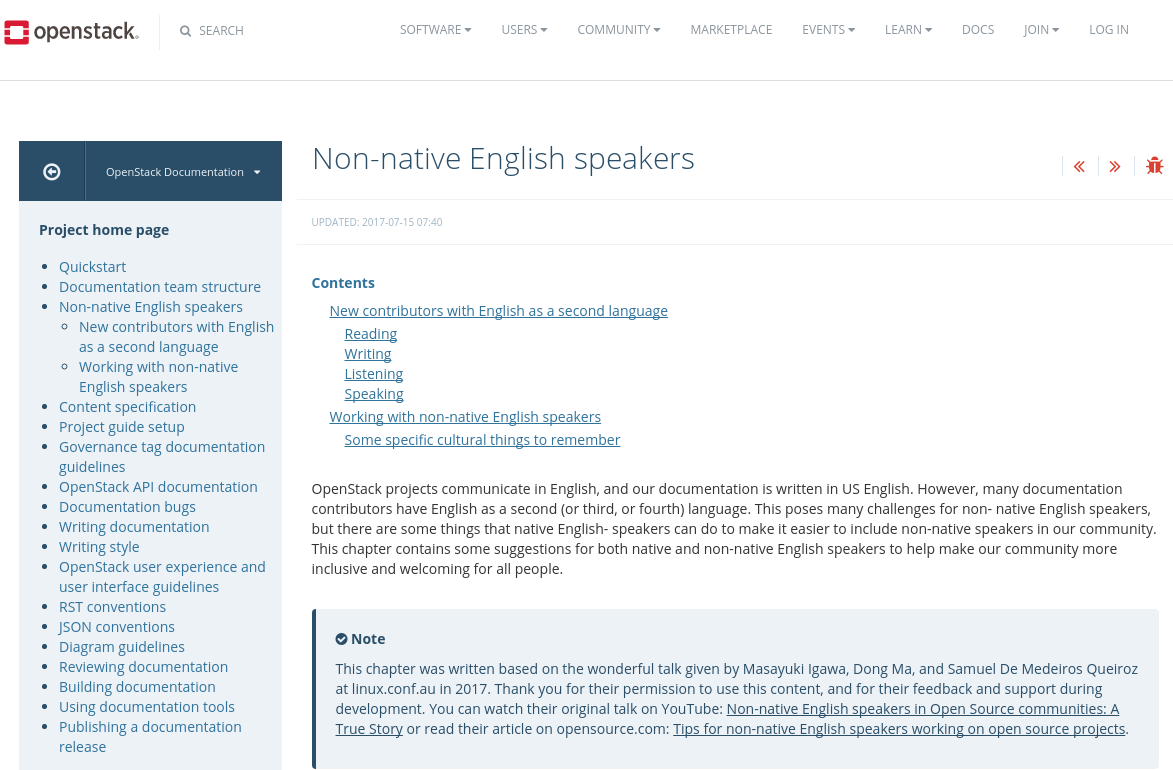
\includegraphics[width=0.492\textwidth]{non-native_English_speakers.png}
    \begin{flushleft}
      \bf\tiny{Image by}\tiny\url{ : opensource.com}
    \end{flushleft}
  \end{center}
\end{frame}


\subsection{Appendix: English version}
\begin{frame}
  \bf\Huge{Appendix: English version}
\end{frame}


\begin{frame}
\frametitle{Japanese - Masayuki}
  \begin{itemize}
    \item NOT to say "Yes / No" clearly
    \item Tend to be perfect
    \item Keep intonation
    \item Size of Economy
    \item Focusing on Reading and Writing
    \item Pronunciation and grammar are very different
      \begin{itemize}
      \item Pronouncing “L” vs “R” in words
      \item Subject-Verb-Object (E) vs Subject-Object-Verb (J)
      \end{itemize}
    \item Katakana: “ネットワーク” = “Network” (English)
    \item Kanji(漢字), Hiragana(ひらがな), Katakana(カタカナ)
    \item Network(ネットワーク), File(ファイル), Comment(コメント), etc..
    \item 和製英語(Japanese-made English): Paso-con(パソコン), Air-con(エアコン), Auto-bi(オートバイ)
      \begin{itemize}
        \item https://en.wikipedia.org/wiki/Wasei-eigo
      \end{itemize}
  \end{itemize}
\end{frame}

\begin{frame}
\frametitle{Chinese}
  \begin{itemize}
  \item Confucian culture
  \item Doctrine of the Mean -  one guideline is Leniency
  \item Like to say yes, don't like to say no
  \item Like to listen, don't like to negotiate
  \item Chinese pronunciation is not understood by others
  \item Not follow well with the English grammar
  \item Writing is hard because of the grammar but it can be understood
  \end{itemize}
\end{frame}

\begin{frame}
\frametitle{Brazilian - Samuel}
  \begin{itemize}
  \item Conversations driven in similar way
  \item Short/direct responses may sound rude
  \item ``i'' (Portuguese) is pronounced as ``e'' (English)
  \item Grammar: adjectives position
  \item Some phonemes do not exist in Portuguese, e.g ``th'' vs ``f''
  \item Regular schools do a poor job teaching English
  \end{itemize}
\end{frame}


\subsection{Language Challenges}
\begin{frame}
  \bf\Huge{Language Challenges}
\end{frame}

\begin{frame}
\frametitle{Reading}
  \begin{itemize}
  \item Easiest in most of the time
  \item One of the most important
  \item IRC conversation goes fast
  \item Long emails, conclusion is unclear
  \end{itemize}
\end{frame}

\begin{frame}
\frametitle{Writing}
  \begin{itemize}
  \item Grammar
  \item Writing long and beautiful sentences is difficult
  \item Simpler sentences are prevalent
  \item Speed in IRC/chat
  \end{itemize}
\end{frame}

\begin{frame}
\frametitle{Listening}
  \begin{itemize}
  \item Variety of accents
  \item Speed
  \item Vocabulary
  \item Grammar
  \item Noisy environments
  \end{itemize}
\end{frame}

\begin{frame}
\frametitle{Speaking}
  \begin{itemize}
  \item Vocabulary
  \item Grammar
  \item Pronunciation
  \item Speed \& Fluency
  \end{itemize}
\end{frame}

\subsection{Overcoming Obstacles}
\begin{frame}
  \bf\Huge{Overcoming Obstacles}
\end{frame}

\begin{frame}
\frametitle{Overcoming Obstacles}
  \begin{itemize}
  \item Cultural challenges harder than language challenges
  \item Language immersion
  \item Forget limitations
  \item Do your best and you will eventually improve
  \item Reading gathers vocabulary
  \item Communicate daily
  \item Useful tools out there
  \item Practice with others or yourself
  \item One-to-one conversations
  \end{itemize}
\end{frame}


\subsection{Onboarding newcomers}
\begin{frame}
  \bf\Huge{Onboarding newcomers}
\end{frame}

\begin{frame}
\frametitle{Newcomers}
  \begin{itemize}
  \item Be friendly
  \item Find a mentor
  \item Share your opinion
  \item Prepare in advance
  \item Ask questions
  \item Brush up your English skills
  \end{itemize}
\end{frame}

\begin{frame}
\frametitle{Native Speakers}
  \begin{itemize}
  \item Be patient
  \item Speak slowly, please
  \item Use simple words and sentences
  \item Encourage communication
  \item Do not make fun
  \end{itemize}
\end{frame}


\end{document}
